\section{Introduction}
\label{sec:introduction}

\looseness=-1 An estimated 7--17\% of recent scientific publications already contain substantial LLM-modified content \cite{mapping_llm_science,monitoring_ai_review}. As these outputs re-enter training corpora \cite{dolma,fineweb} and seed further generation, text accumulates at varying \emph{generation depths}; each successive cycle reshapes distributional properties in ways that matter for data provenance, corpus auditing, and contamination monitoring in base-model pretraining corpora \cite{ccnet,dsir} as well as model collapse analysis \cite{curse_of_recursion,strong_model_collapse}. Understanding \emph{how} recursive generation alters text distributions, and which properties change versus which are preserved, is therefore a prerequisite for principled corpus curation, yet current methods address only binary human-or-machine detection \cite{detectgpt,fast_detectgpt,binoculars,ld_score}.
Base models provide the cleanest substrate to isolate depth effects from alignment-induced changes.
We find that recursive generation produces a decomposable depth profile: distributional \emph{location} drifts with depth while \emph{shape} remains stable across generators, an asymmetry sufficient for cross-generator depth prediction.

\looseness=-1 Distributional compression under recursive generation is well-documented \cite{curious_decline,broken_telephone,markovian_chains}, yet existing analyses characterize \emph{that} and \emph{why} convergence occurs without decomposing what drifts from what is preserved.
We introduce \emph{depth profiling} (coarse ordinal classification into gen-0\,/\,gen-1\,/\,gen-2+) and decompose this compression into structurally distinct components.
Across eight base-model generators spanning five architectural families (0.6B--8B), the NLL distribution's central tendency---mean entropy (per-token NLL under a fixed reference model, not information-theoretic entropy; \S\ref{sec:features}) and lexical diversity---drifts monotonically with depth, while its shape (entropy extremes, tail structure) remains ${\geq}8{\times}$ more stable ($d{=}0.74$--$1.05$ vs.\ $d < 0.10$; entropy std is intermediate at $d{=}0.46$).
We term this location/shape asymmetry the \emph{differential depth response} (DDR; Figure~\ref{fig:ddr-trajectory}), an empirical regularity of base-model autoregressive generation that is mechanistically distinct from model collapse \cite{curse_of_recursion}. Model collapse erodes tail coverage via weight updates; DDR instead analyzes fixed-parameter inference chains.
The stationary shape component complements location drift for depth prediction without per-generator calibration.

\begin{figure*}[t!]
\centering
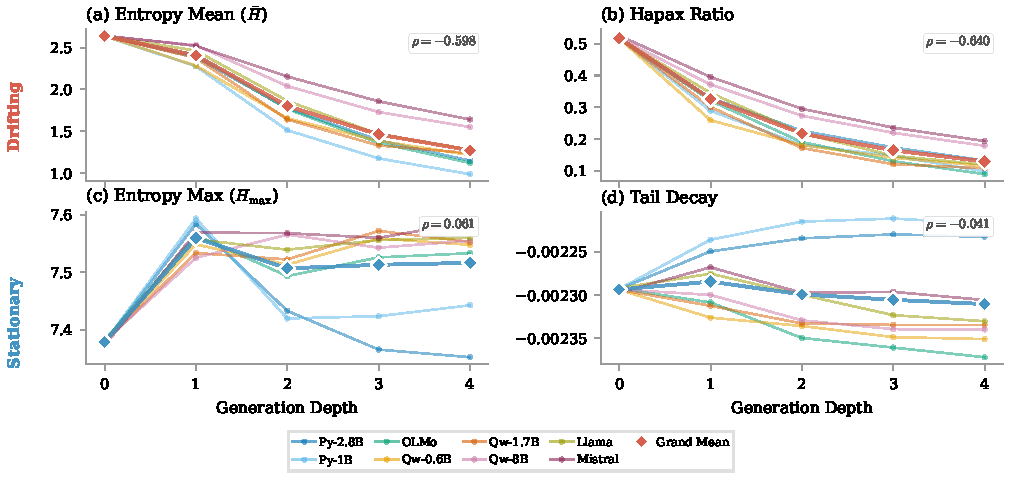
\includegraphics[width=\textwidth]{fig_ddr_trajectory.pdf}
\caption{Feature trajectories across generation depth ($y$-axis: $z$-scored feature values). \textbf{Top row (drifting)}: entropy mean and hapax ratio decline monotonically across all eight generators ($|\rho| > 0.59$). \textbf{Bottom row (stationary)}: entropy max and tail decay remain flat ($|\rho| < 0.07$). Colored lines: individual generators; diamonds: cross-generator mean (red for drifting, blue for stationary). This dichotomy defines the DDR.}
\label{fig:ddr-trajectory}
\end{figure*}
We focus on base (pretrained) models; instruction tuning degrades depth signal (Appendix~\ref{app:instruct}).
Figure~\ref{fig:framework} summarizes the pipeline: recursive generation chains (\S\ref{sec:generation}), feature extraction with DDR partitioning (\S\ref{sec:features}), and leave-one-generator-out (LOGO) evaluation (\S\ref{sec:evaluation}).

\looseness=-1 As a proof of concept, a lightweight 7-feature ensemble informed by DDR achieves leak-free binary F1\,=\,0.694 (macro-averaged LOGO; pooled: 0.705), matching multi-detector ensembles (0.708) at ${\sim}2.4\times$ lower cost; an end-to-end QLoRA \cite{qlora} (Quantized Low-Rank Adaptation) classifier reaches 3-class F1\,=\,0.905 (within-model 5-fold CV; Appendix~\ref{app:qlora}), and the depth signal thus extends well beyond handcrafted features.

Our contributions:
\begin{enumerate}[nosep,leftmargin=*]
    \item \textbf{Empirical decomposition (DDR).} Across eight generators from five families, we decompose inference-chain drift into two primary response zones (drifting, $d{=}0.74$--$1.05$; near-stationary, $d < 0.10$) plus one intermediate feature ($d{=}0.46$). Where prior work documents \emph{what converges} \cite{curious_decline,markovian_chains}, DDR identifies \emph{what is approximately preserved}, an empirical regularity with analytical utility for depth classification without per-generator calibration.
    \item \textbf{Task formulation and evaluation suite.} We define generation depth classification as an ordinal prediction task and construct a controlled dataset of 37K texts from eight generators across five families (0.6B--8B; exploratory evidence extends to 14B, Appendix~\ref{app:9gen-scale}), with leave-one-generator-out cross-validation as the primary evaluation protocol.
    \item \textbf{Scope characterization.} Systematic evaluation across temperature, prompt type, instruction tuning, model scale, domain transfer, and perturbation robustness maps the operational envelope of depth profiling.
\end{enumerate}

\begin{figure*}[t]
\centering
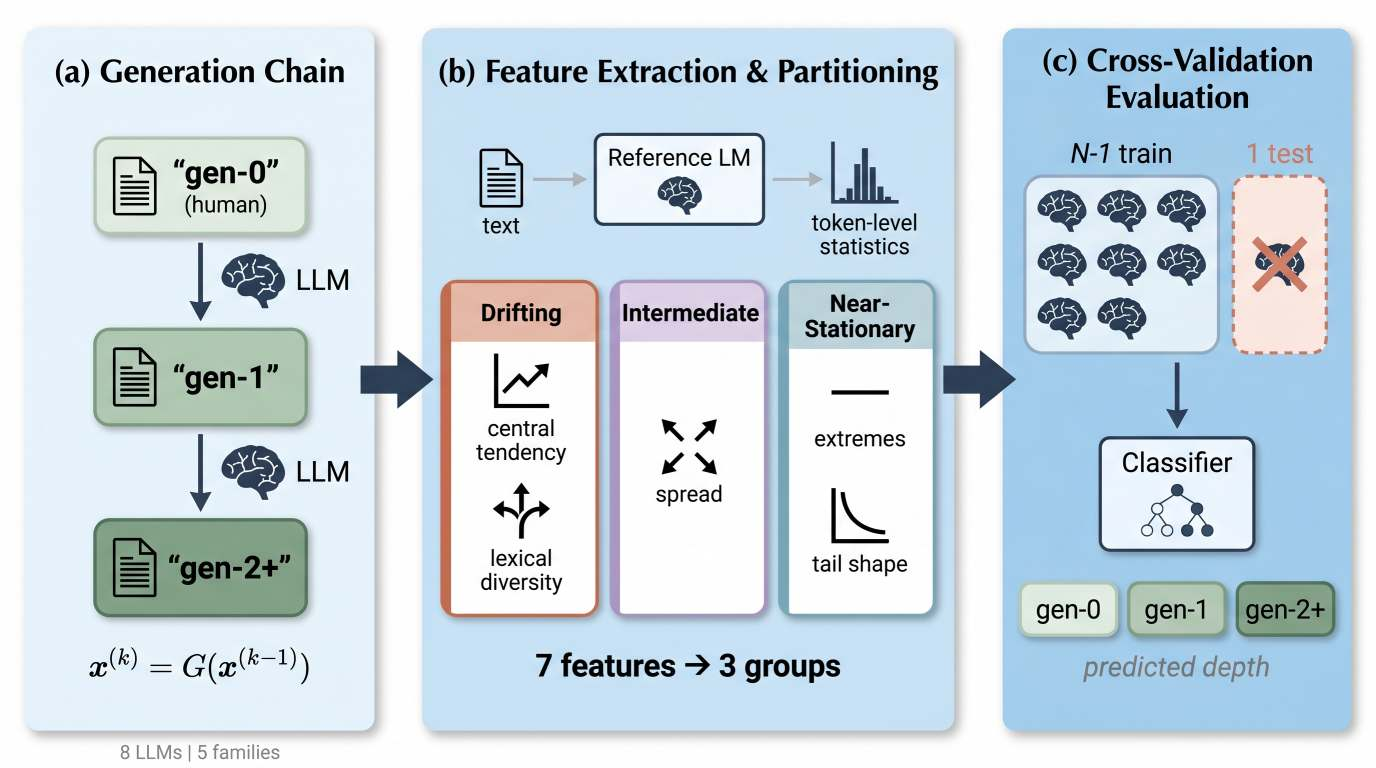
\includegraphics[width=\textwidth]{fig2_framework.pdf}
\caption{Depth profiling pipeline. (a)~Human seeds are iteratively fed through generator $G$ to produce chains of increasing depth. (b)~Seven features extracted from NLL distributions group into three DDR zones: drifting (red), intermediate (purple), near-stationary (blue). (c)~LOGO evaluation holds out one generator for testing.}
\label{fig:framework}
\end{figure*}
